\documentclass[11pt]{article}
\usepackage{amssymb,graphicx,amsmath,mathtools,float}
\usepackage{lscape}
\usepackage[utf8]{inputenc}
\usepackage[spanish, es-tabla]{babel}

\usepackage{indentfirst}	% Tabular tras un section
\usepackage{hyperref}
\hypersetup{
	colorlinks=false,
	citecolor=black,
	filecolor=black,
	linkcolor=red,
	urlcolor=black,
	pdfborderstyle={/S/U/W 1}
}

\usepackage[svgnames]{xcolor}
\definecolor{griscaption}{RGB}{100,100,100}
\usepackage{caption}
\usepackage[font={color=griscaption},figurename=Fig.,labelfont={bf}]{caption}


\newtheorem{theorem}{Theorem}
\newtheorem{corollary}[theorem]{Corollary}
\newtheorem{lemma}[theorem]{Lemma}
\newtheorem{proposition}[theorem]{Proposition}
\newtheorem{definition}[theorem]{Definición}

\newcommand\ddfrac[2]{\frac{\displaystyle #1}{\displaystyle #2}}







\title{Determinación de Órbitas Elípticas}
\author{Simón López
\\
{\small Matemáticas e Ingeniería Informática}
\\
{\small Universidad de Granada, 18071 Granada, Spain}
\\
{\small simondelosbros@correo.ugr.es}}
\date{\today}
\setlength{\unitlength}{1cm}
\setlength{\unitlength}{1cm}


\begin{document}


\section{Método Laplaciano de Determinación}

\subsection{\normalfont{\textit{Determinar el valor de la primera y segunda derivada de $\lambda$, $\mu$, $\nu$, $X$, $Y$, $Z$ en algún momento $t$.}}}
\label{subsec:primera_segunda_derivada}
Dado que no podemos calcular el valor exacto de la derivada de $\lambda$, $\mu$ y $\nu$, utilizaremos fórmulas de derivación numérica con dos nodos para obtener un valor aproximado de éstas. Tomemos, por ejemplo, $t=t_2$, que por el momento nos bastará para demostrar que se puede realizar una buena aproximación. Supongamos que el valor de $\lambda'$ no cambia muy rápido; entonces, el valor de ésta en medio del intervalo $[t_1,t_2]$ será muy cercano al valor de:
\[
\lambda_{12}'=\frac{\lambda_2-\lambda_1}{t_2-t_1},
\]

\noindent y dado que los nodos elegidos cumplen $t_2>t_1$, estaremos ante una diferencia regresiva. Análogamente podremos determinar el valor de $\lambda_{23}'$.\\

El error de estas aproximaciones, suponiendo que $\lambda$ sea de clase 2 en el intervalo de aproximación, es del orden de $(t_2-t_1)$ y $(t_3-t_2)$ para $\lambda_{12}'$ y $\lambda_{23}'$ respectivamente. Por tanto, cuanto más pequeño sea el intervalo donde realizamos las operaciones, mejor será la aproximación obtenida. Además, si la longitud del intervalo $[t_1,t_2]$ es igual a la longitud de $[t_2,t_3]$, podremos calcular el valor aproximado de $\lambda'$ en $t_2$ mediante una diferencia centrada, obteniendo:
\[
\lambda'_2=\frac{\lambda_{12}'+\lambda_{23}'}{2}
\]

\noindent es decir, la media de los dos valores calculados anteriormente. Si los intervalos tienen una longitud diferente, podremos ajustar la disparidad entre ellos para realizar la aproximación.\\

Análogamente, podremos definir la derivada segunda de $\lambda$ en $t_2$ de manera aproximada como:
\[
\lambda''_2=\frac{\lambda_{23}'-\lambda_{12}'}{\frac{1}{2}(t_3-t_1)}
\]

\noindent de orden $(t_3-t_1)^2$ siempre que $\lambda\in\mathcal{C}^4[t_1,t_3]$. Utilizaremos el mismo método para calcular la primera y segunda derivada de $\mu$ y $\nu$, y podemos suponer que las tres funciones son de clase infinito en todo $\mathbb{R}$.\\

Como hemos comentado antes, las aproximaciones obtenidas de esta manera serán más cercanas cuanto menor sea la longitud de los intervalos entre las observaciones, y generalmente, en la práctica, los intervalos que utilizaremos serán cortos.\\

Finalmente, para calcular la primera y segunda derivada de $X$, $Y$ y $Z$ utilizaremos la efemérides proporcionada por el \href{https://ssd.jpl.nasa.gov/horizons.cgi}{\textit{Jet Propulsion Laboratory}} en su página web, que nos dará el valor de estas variables para cualquier día del año\footnote{Mientras que el JPL proporciona una herramienta para generar efemérides, hemos de tener en cuenta que no podemos escoger una posición exacta de observación en la Tierra. Para ello, podemos utilizar \href{http://xjubier.free.fr/en/site_pages/astronomy/ephemerides.html}{\textit{esta}} página.}.\\

\subsection{\normalfont{\textit{Imponer la condición de que $C$ gira en torno a $S$ de acuerdo a la ley de gravitación.}}}
\label{subsec:ley_gravitacion}
Asumiendo que el cuerpo observado $C$ no está alterado por la interacción con otros cuerpos cercanos, podemos asegurar que cumplirá siguientes ecuaciones diferenciales:
\begin{align}
\left\{
\def\arraystretch{2}
\begin{array}{l}
	\ddfrac{d^2x}{dt^2}=-\ddfrac{k^2x}{r^3}\\
	\ddfrac{d^2y}{dt^2}=-\ddfrac{k^2y}{r^3}\\
	\ddfrac{d^2z}{dt^2}=-\ddfrac{k^2z}{r^3}
\end{array}
\right.
\label{eq:ley_gracitacion_C}
\end{align}

\noindent donde $k^2=GM$, $G=6.674\times10^{-11}\frac{\text{N}\cdot\text{m}^2}{\text{kg}^2}$ constante de gravitación y $M=1.989\times10^{30}\;\text{kg}$ masa del Sol. Tomamos solo la masa del Sol, $M$, ya que la masa de nuestro cuerpo es despreciable en comparación con ésta usando como modelo el problema de Kepler.\\

Además, utilizando las \hyperref[eq:terminologia]{relaciones entre $E$, $C$ y $S$}, así como los resultados vistos anteriormente, llegamos a:
\begin{align}
\left\{
\begin{array}{l}
	x=\rho\lambda-X\\
	y=\rho\mu-Y\\
	z=\rho\nu-Z
\end{array}
\right.
\label{eq:relacion_C_S_E}
\end{align}

\noindent y sustituyendo los valores obtenidos en las  ecuaciones \eqref{eq:ley_gracitacion_C}, obtenemos lo siguiente:
\begin{align}
\left\{
\def\arraystretch{2}
\begin{array}{l}
	(\rho\lambda)'' - X'' = \ddfrac{-k^2(\rho\lambda-X)}{r^3}\\
	(\rho\mu)'' - Y'' = \ddfrac{-k^2(\rho\mu-Y)}{r^3}\\
	(\rho\nu)'' - Z'' = \ddfrac{-k^2(\rho\nu-Z)}{r^3}
\end{array}
\right.
\label{eq:derivada_segunda}
\end{align}

Desarrollando la segunda derivada de $\rho\lambda$ conseguimos:
\[
(\rho\lambda)''=(\rho'\lambda+\rho\lambda')'=\rho''\lambda+2\rho'\lambda'+\rho\lambda'',
\]

\noindent valor que utilizaremos más adelante.\\

De la misma manera que hemos hecho con $C$, escribimos las ecuaciones de gravitación para $E$, que gira alrededor de $S$ en concordancia con la ley de gravitación universal.
\begin{align}
\left\{
\def\arraystretch{2}
\begin{array}{l}
	X'' = -\ddfrac{k^2X}{R^3}\\
	Y'' = -\ddfrac{k^2Y}{R^3}\\
	Z'' = -\ddfrac{k^2Z}{R^3}
\end{array}
\right.
\label{eq:ley_gravitacion_E}
\end{align}\\

Utilizando este resultado, sustituyendo en la ecuación \eqref{eq:derivada_segunda} y desarrollando llegamos a lo siguiente:
\begin{align}
\left\{
\def\arraystretch{2}
\begin{array}{l}
	\lambda\rho''+2\lambda'\rho'+[\lambda''+\ddfrac{k^2\lambda}{r^3}]\rho=-k^2X[\ddfrac{1}{R^3}-\ddfrac{1}{r^3}]\\
	\mu\rho''+2\mu'\rho'+[\mu''+\ddfrac{k^2\mu}{r^3}]\rho=-k^2Y[\ddfrac{1}{R^3}-\ddfrac{1}{r^3}]\\
	\nu\rho''+2\nu'\rho'+[\nu''+\ddfrac{k^2\nu}{r^3}]\rho=-k^2Z[\ddfrac{1}{R^3}-\ddfrac{1}{r^3}]
\end{array}
\right.
\label{eq:fundamental_equations}
\end{align}

Así, las incógnitas de las ecuaciones pasan a ser $r, \; \rho, \; \rho'$ y $\rho''$.\\

\subsection{\normalfont{\textit{Determinar la Distancia de $C$ desde $E$ y $S$}}}
\label{subsec:distancias}
Para resolver este paso, utilizaremos las ecuaciones que hemos acabado obteniendo del paso anterior, \eqref{eq:fundamental_equations}, y una condición geométrica que cumplirán los tres cuerpos. Para ello, tomaremos el sistema \eqref{eq:fundamental_equations} como un sistema lineal en $\rho, \rho'$ y $\rho''$ y resolveremos utilizando la regla de Cramer. Comencemos definiendo el siguiente determinante:

\[
D =
\left|
\begin{array}{ccc}
	\lambda & 2\lambda' & \lambda''+\frac{k^2\lambda}{r^3}\\
	\mu & 2\mu' & \mu''+\frac{k^2\mu}{r^3}\\
	\nu & 2\nu' & \nu''+\frac{k^2\nu}{r^3}
\end{array}
\right|
=
2
\left|
\begin{array}{ccc}
	\lambda & \lambda' & \lambda''\\
	\mu & \mu' & \mu''\\
	\nu & \nu' & \nu''
\end{array}
\right|
=2W(\lambda,\mu,\nu)
\]

\noindent siendo $W(\lambda,\mu\nu)$ el Wronskiano de las coordenadas angulares.\\

Esta segunda forma del determinante la obtenemos mediante la transformación $C_3-\frac{k^2\lambda}{r^3}C_1$ sobre la matriz, donde $C_i$ representará la columna i-ésima. Una vez hayamos sustituido las derivadas exactas por su valor aproximado calculado anteriormente, conoceremos todas las cantidades de este determinante.\\

Por otra parte, definiremos el determinante $D_1$, que utilizaremos para calcular $\rho$ mediante la regla de Cramer, reemplazando la tercera columna por los términos independientes del sistema \eqref{eq:fundamental_equations} y omitiendo el factor $[\frac{1}{R^3}-\frac{1}{r^3}]$, conociendo de nuevo todas las cantidades utilizadas. Así, obtenemos el siguiente determinante:
\[
D_1 = -2k^2
\left|
\begin{array}{ccc}
\lambda & \lambda' & X\\
\mu & \mu' & Y\\
\nu & \nu' & Z
\end{array}
\right|
\]

Con todo esto, la distancia $\rho$ se determina por
\[
\rho = \frac{D_1}{D}[\frac{1}{R^3}-\frac{1}{r^3}],
\]

El valor de $r$ es desconocido, por lo que añadiremos la siguiente ecuación formando con las dos un sistema de ecuaciones en $r$ y $\rho$.
\[
r^2=\rho^2+R^2-2\rho R\cos(\psi),
\]

\noindent donde $\psi$ es el ángulo formado en $E$ trazando una línea imaginaria hasta el Sol y hasta el cuerpo observado, es decir, entre $R$ y $\rho$; esta ecuación expresa el hecho de que $S$, $E$ y $C$ forman un triángulo como vimos en la \hyperref[figure:1]{figura 1}.\\

Dado que disponemos de los valores $\overrightarrow{SE}=(X,Y,Z)$ y $\overrightarrow{EC}=(\lambda,\mu,\nu)$, vector unitario, podremos obtener el coseno de $\psi$ con:
\[
\cos{\psi}=\frac{\langle\overrightarrow{SE},\overrightarrow{EC}\rangle}{|\overrightarrow{SE}||\overrightarrow{EC}|}=\frac{\langle(X,Y,Z),(\lambda,\mu,\nu)\rangle}{R}
\]

Resolviendo el sistema de ecuaciones al que hemos llegado obtendremos los valores de $\rho$ y $r$, habiendo terminado este paso. Más adelante discutiremos la unicidad de la solución en el sistema con $r,\rho>0$ (\ref{subsec:unicidad}). Al solucionar este problema, podremos calcular las coordenadas de $C$ mediante las ecuaciones \eqref{eq:relacion_C_S_E} de las relaciones entre $S$, $E$ y $C$.\\

\subsection{\normalfont{\textit{Determinación de las Componentes de Velocidad de $C$}}}
\label{subsec:velocity_component}
Se sigue de las ecuaciones \eqref{eq:relacion_C_S_E} que:
\[
\left\{
\begin{array}{l}
	x'=\rho'\lambda+\rho\lambda'-X'\\
	y'=\rho'\mu+\rho\mu'-Y'\\
	z'=\rho'\nu+\rho\nu'-Z'
\end{array}
\right.	
\]

En estas ecuaciones solo tenemos una incógnita, $\rho'$, que podremos determinar resolviendo por Cramer en \eqref{eq:fundamental_equations} a partir de:
\[
\rho'=+\frac{D_2}{D}[\frac{1}{R^3}-\frac{1}{r^3}],
\; \; \; \; \; \; \; \; \; \text{ con } \;
D_2 = -k^2
\left|
\begin{array}{ccc}
\lambda & X & \lambda''\\
\mu & Y & \mu''\\
\nu & Z & \nu''
\end{array}
\right|
\]

Notar que en $D_2$ también hemos realizado la operación $C_3-\frac{k^2\lambda}{r^3}C_1$, como en $D$, para obtener un determinante más simple.\\

Así, $x'$, $y'$ y $z'$ se vuelven conocidas.\\

\subsection{\normalfont{\textit{Determinar los elementos de la órbita a partir de la posición y los componentes de velocidad del cuerpo observado}}}
\label{subsec:elements_determination}
Una vez conocida tanto la posición como la velocidad del cuerpo en un instante determinado, nos dispondremos a calcular los elementos orbitales mediante las distintas fórmulas estudiadas en el manual de Mecánica Celeste\cite{ortega}. Denotemos por $x(t)=(x,y,z)(t)$ la posición del objeto y $x'(t)$ su derivada, la velocidad.\\

Comencemos determinando la energía que tiene nuestro cuerpo en un instante $t$. Para ello utilizaremos:
\[
h=\frac{|x'(t)|^2}{2}-\frac{\mu}{|x(t)|}
\]

\noindent donde $\mu=GM$ una constante positiva. Con el valor de la energía podemos pasar a calcular la primera de nuestros elementos astronómicos, la longitud del semieje mayor, $a$, utilizando la siguiente ecuación:
\[
a=-\frac{\mu}{2h}
\]

Pasemos ahora a calcular el momento angular de nuestro objeto. Dado que la masa del objeto observado es despreciable frente a la masa del Sol, podremos obviar su valor, obteniendo así el vector del momento angular mediante:
\[
c=x(t)\wedge x'(t)
\]

Calculado el momento angular, podremos obtener el vector de excentricidad para la órbita del cuerpo observado:
\[
\vec{e}=-\frac{x(t)}{|x(t)}-\frac{1}{\mu}(c\wedge x'(t))
\]

\noindent y la excentricidad de la órbita será $e=|\vec{e}|$.\\

Una vez obtenidos estos valores, podemos utilizar la tercera ley de Kepler para obtener el período mínimo (suponiendo que nuestra órbita se corresponda con la de una elipse). Si el momento angular del objeto observado $c\neq0$ y su energía $h<0$, entonces la órbita es periódica y su período mínimo valdrá:
\[
p=\frac{2\pi}{\sqrt{\mu}}a^{3/2}
\]

Sabemos que el vector del momento angular, del que disponemos, es el vector normal al plano orientado de la órbita, pudiendo calcular así la inclinación del plano de movimiento. Además, calculando la intersección de éste con el plano de la eclíptica obtenemos la línea de nodos y con ella el nodo ascendente $\mathcal{N}_+$, con la que podremos determinar $\Omega$.
\[
\left\{
\begin{array}{l}
	i=\measuredangle(\vec{e}_3,\vec{n}), \; \; \; \; \; \; \; \; \; \; i\in]0,\pi[\\
	\Omega=\measuredangle(\vec{e}_1, \mathcal{N}_+), \; \; \; \; \; \Omega\in\mathbb{R}/2\pi\mathbb{Z}
\end{array}
\right.
\]

Finalmente usaremos el vector de excentricidad $\vec{e}$ para calcular $\omega$, utilizando el nodo ascendente como eje de rotación.\\

\subsection{\normalfont{\textit{Determinación de $\lambda$, $\mu$ y $\nu$ y sus derivadas mediante series de potencias}}}
\label{subsec:series_potencias}
Tal y como hemos visto en la sección \ref{subsec:primera_segunda_derivada}, hemos de calcular la primera y segunda derivada de las coordenadas angulares o de $\lambda$, $\mu$ y $\nu$. Definimos el valor $\tau=k(t-t_0)$ con el que podemos reescribir las ecuaciones \eqref{eq:ley_gracitacion_C} como vemos a continuación:
\begin{align}
\left\{
\def\arraystretch{2}
\begin{array}{l}
	\ddfrac{d^2x}{d\tau^2}=-\ddfrac{x}{r^3}\\
	\ddfrac{d^2y}{d\tau^2}=-\ddfrac{y}{r^3}\\
	\ddfrac{d^2z}{d\tau^2}=-\ddfrac{z}{r^3}
\end{array}
\right.
\label{eq:ley_gravitacion_C_2}
\end{align}

La solución para estas ecuaciones diferenciales de segundo orden puede ser expandida como serie de Taylor en $\tau$, y esta convergerá si el valor de $\tau$ no es especialmente grande.
\begin{align}
\left\{
\def\arraystretch{1.5}
\begin{array}{l}
	x=x_0+x_0'\tau+\frac{1}{2}(\frac{d^2x}{d\tau^2})_0\tau^2+...+\frac{1}{n!}(\frac{d^nx}{d\tau^n})_0\tau^n+...\\
	y=y_0+y_0'\tau+\frac{1}{2}(\frac{d^2y}{d\tau^2})_0\tau^2+...+\frac{1}{n!}(\frac{d^ny}{d\tau^n})_0\tau^n+...\\
	z=z_0+x_0'\tau+\frac{1}{2}(\frac{d^2z}{d\tau^2})_0\tau^2+...+\frac{1}{n!}(\frac{d^nz}{d\tau^n})_0\tau^n+...\\	
\end{array}
\right.
\label{eq:series_taylor}
\end{align}

\noindent donde con el subíndice 0 estaremos indicando que los valores se toman en $\tau=0$. Podemos sustituir la segunda derivada que aparece en estas series por su valor en \eqref{eq:ley_gracitacion_C_2}, la tercera derivada por la derivada de ésta y a partir de la cuarta derivada repetimos este proceso, teniendo así que las series estarán solo en función de la $x$, $y$, $z$ y la primera derivada de cada una de estas, todos ellas tomadas en $\tau=0$.  De esta manera llegamos al hecho de que la solución $x$, $y$, $z$ del problema de Kepler es una función analítica, pues su serie de Taylor centrada en $\tau$ converge a la función en un entorno de éste para cualquier $\tau$ que elijamos.\\

Hemos de tener en cuenta que el valor de estas series no siempre tiene valor práctico, pues el intervalo de tiempo para la convergencia puede ser demasiado grande; notar que los límites serán más pequeños cuanto más pequeña sea la distancia del perihelio y más grande la excentricidad de nuestra órbita, y dependerán de la posición del cuerpo en $\tau=0$.\\

En el caso de la Tierra, expandiendo sus coordenadas en series de potencias, obtendremos una convergencia durante largos intervalos de tiempo debido a la pequeña excentricidad de la órbita terrestre ($e\approx0.0167$). Así, se sigue de la ecuación \eqref{eq:relacion_C_S_E}, que relaciona las coordenadas de la Tierra, el Sol y el cuerpo observado que las ecuaciones de $\rho$, $\lambda$, $\mu$ y $\nu$ también son funciones analíticas y por ello podrán ser expandidas como series de Taylor, con el mismo rango de utilidad que el de las series para $x$, $y$ y $z$.\\

Veamos las series para $\lambda$, pues las de $\mu$ y $\nu$ serán simétricamente similares. Definimos $\tau_1$, $\tau_2$ y $\tau_3$ como los valores de $\tau$ tomando $t_1$, $t_2$ y $t_3$ respectivamente. Así, las series para $\lambda$ son:
\begin{align}
\left\{
\begin{array}{l}
\lambda=c_0+c_1\tau+c_2\tau^2+...\\
\lambda_1=c_0+c_1\tau_1+c_2\tau_1^2+...\\
\lambda_2=c_0+c_1\tau_2+c_2\tau_2^2+...\\
\lambda_3=c_0+c_1\tau_3+c_2\tau_3^2+...
\end{array}
\right.
\label{eq:series_lambda}
\end{align}

\noindent donde los valores $c_0, c_1, c_2, ...$ son constantes. Si estas series terminan tras los términos elevados al cuadrado, podremos determinar $c_0$, $c_1$ y $c_2$ resolviendo como un sistema de ecuaciones, ya que conocemos las cantidades $\lambda_1$, $\lambda_2$, $\lambda_3$. Así, tenemos que cuantas más observaciones tengamos disponibles, más coeficientes podrán ser determinados.\\

Para expresar $\lambda$ en términos de $\tau$ tomando solo coeficientes conocidos, igualaremos a 0 la resultante de $1$, $c_0$, $c_1$ y $c_2$, y obtendremos lo siguiente:
\begin{align}
\left|
\begin{array}{cccc}
\lambda & 1 & \tau & \tau^2\\
\lambda_1 & 1 & \tau_1 & \tau^2_1\\
\lambda_2 & 1 & \tau_2 & \tau^2_2\\
\lambda_3 & 1 & \tau_3 & \tau^2_3\\
\end{array}
\right|
=0
\label{eq:resultante}
\end{align}

Resolvemos este determinante desarrollando por la primera columna y despejando $\lambda$ obtenemos:
\begin{align}
\lambda=
\frac{(\tau-\tau_2)(\tau-\tau_3)}{(\tau_1-\tau_2)(\tau_1-\tau_3)}\lambda_1
+\frac{(\tau-\tau_3)(\tau-\tau_1)}{(\tau_2-\tau_3)(\tau_2-\tau_1)}\lambda_2
+\frac{(\tau-\tau_1)(\tau-\tau_2)}{(\tau_3-\tau_1)(\tau_3-\tau_2)}\lambda_3
\label{eq:lambda_value}
\end{align}

\noindent obteniendo así el polinomio de interpolación de Lagrange para $\lambda$. Hemos de tener en cuenta que los valores de $\tau_1$, $\tau_2$ y $\tau_3$ han de ser diferentes entre sí para que no se anulen los denominadores.\\

Con esto, somos capaces de obtener $\lambda$ de manera exacta en $\tau_1$, $\tau_2$ y $\tau_3$; para otros valores más pequeños de $\tau$ obtendremos $\lambda$ de forma aproximada. Para obtener un valor exacto de $\lambda$ habremos de tomar la primera ecuación de \eqref{eq:series_lambda}, una serie infinita, dentro de su rango de convergencia. Considerando esta serie geométricamente podemos definir una curva que llamaremos $C$; por otra parte definiremos la curva $C_2$ como la que produce el polinomio de interpolación \eqref{eq:lambda_value}. Representando las dos en una misma gráfica podemos visualizar la diferencia entre el valor real y el aproximado mediante interpolación de las funciones estudiadas:
\begin{figure}[H]
\centering
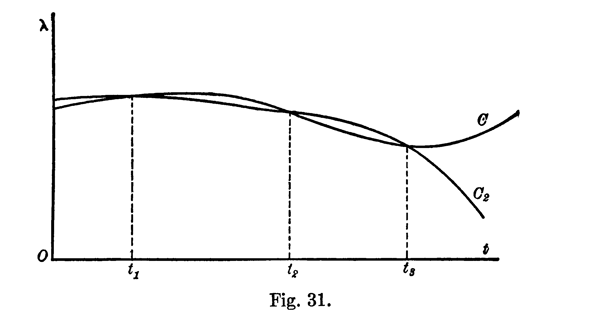
\includegraphics[scale=0.5]{images/fig_31.png}
\end{figure}

Dichas curvas se intersecan en $\tau_1$, $\tau_2$ y $\tau_3$, y en general en ningún otro punto; tomando valores pequeños de $\tau$ las dos curvas casi coincidirán.\\

Con el hecho anterior y todos los vistos anteriormente, podemos justificar que los valores de $\tau$ han de ser pequeños en la práctica para que las cantidades aproximadas calculadas sean lo más cercanas a su valor original. Además, no tendría sentido una diferencia de tiempo muy grande entre las observaciones del objeto, pues pasaríamos mucho tiempo para determinar una única órbita.\\

Por último, ya que necesitamos la primera y segunda derivada de $\lambda$, nos bastará con derivar del polinomio \eqref{eq:lambda_value}.
\begin{align*}
\lambda' = \frac{2\tau-(\tau_2+\tau_3)}{(\tau_1-\tau_2)(\tau_1-\tau_3)}\lambda_1
+\frac{2\tau-(\tau_3+\tau_1)}{(\tau_2-\tau_3)(\tau_2-\tau_1)}\lambda_2
+\frac{2\tau-(\tau_1+\tau_2)}{(\tau_3-\tau_1)(\tau_3-\tau_2)}\lambda_3\\
\lambda'' = \frac{2}{(\tau_1-\tau_2)(\tau_1-\tau_3)}\lambda_1
+\frac{2}{(\tau_2-\tau_3)(\tau_2-\tau_1)}\lambda_2
+\frac{2}{(\tau_3-\tau_1)(\tau_3-\tau_2)}\lambda_3
\end{align*}

Tal y como comentamos anteriormente, se procederá al cálculo de $\mu$ y $\nu$ de manera similar a la desarrollada anteriormente.

\newpage


\section{Estudio de la unicidad de la solución}

\subsection{\normalfont{\textit{Ecuaciones fundamentales en el método de Laplace}}}
\label{subsec:fundamental_equations}
Para terminar la explicación del método de determinación con tres observaciones, recapitulemos viendo las principales ecuaciones utilizadas para obtener la órbita del objeto observado. Las ecuaciones fundamentales serán las de \eqref{eq:fundamental_equations}, que involucrarán las coordenadas angulares $\lambda$, $\mu$, $\nu$ y sus derivadas, las cuáles conocemos su valor aproximado por \ref{subsec:primera_segunda_derivada} o \ref{subsec:series_potencias}. Por otra parte, el valor de $\rho$ y sus derivadas se obtendrá resolviendo las ecuaciones fundamentales utilizando la regla de Cramer, como vimos en anteriores apartados. Nos faltaría por calcular $\rho''$, donde el determinante para el numerador es el siguiente: 
\[
\left|
\begin{array}{ccc}
-k^2X & 2\lambda' & \lambda''+\frac{k^2\lambda}{r^3}\\
-k^2Y & 2\mu' & \mu''+\frac{k^2\mu}{r^3}\\
-k^2Z & 2\nu' & \nu''+\frac{k^2\nu}{r^3}
\end{array}
\right|
=-2k^2
\left|
\begin{array}{ccc}
X & \lambda' & \lambda''\\
Y & \mu' & \mu''\\
Z & \nu' & \nu''
\end{array}
\right|
-\frac{2k^4}{r^3}
\left|
\begin{array}{ccc}
X & \lambda' & \lambda\\
Y & \mu' & \mu\\
Z & \nu' & \nu
\end{array}
\right|
=
D_3-\frac{k^2D_1}{r^3}
\]

El signo negativo delante del determinante $D_1$ aparece por intercambiar la primera y la tercera columna del determinante inmediatamente anterior.\\

Así, tenemos que los valores de $\rho$ y sus derivadas pueden ser calculados mediante:
\begin{align}
\left\{
\def\arraystretch{1.5}
\begin{array}{l}
	\rho   = \ddfrac{D_1}{D}[\ddfrac{1}{R^3}-\ddfrac{1}{r^3}]\\
	\rho'  = \ddfrac{D_2}{D}[\ddfrac{1}{R^3}-\ddfrac{1}{r^3}]\\
	\rho'' = \ddfrac{D_3}{D}[\ddfrac{1}{R^3}-\ddfrac{1}{r^3}]
\end{array}
\right.
\label{eq:rho_values}
\end{align}

\noindent con $D$, $D_1$ y $D_2$ definidos anteriormente.\\

Los determinantes $D$, $D_1$, $D_2$, $D_3$ están sujetos a pequeños errores dado que los valores implicados en ellos están calculados de forma aproximada, aunque dichos errores podrán ser corregidos tras calcular de forma aproximada el valor de $\rho$ y $\rho'$ con las ecuaciones superiores. Además, trabajamos bajo el supuesto de que las observaciones al objeto son realizadas desde el centro de la Tierra, y no desde un punto concreto de ella. Tras haber calculado de forma aproximada las distancias podremos corregir dichas observaciones por los efectos de la posición del observador sobre un punto en la superficie de la Tierra.\\


\subsection{\normalfont{\textit{Ecuaciones para la determinación de las distancias $r$ y $\rho$}}}
\label{subsec:distancias_r_rho}
Recordemos la imagen \ref{fig:notation} en la que mostrábamos el triángulo formado por los tres cuerpos $S$, $E$ y $C$ junto a sus distancias. Definamos $\psi$ y $\phi$, ángulos formados en $E$ y $C$ respectivamente.

\begin{figure}[H]
\centering
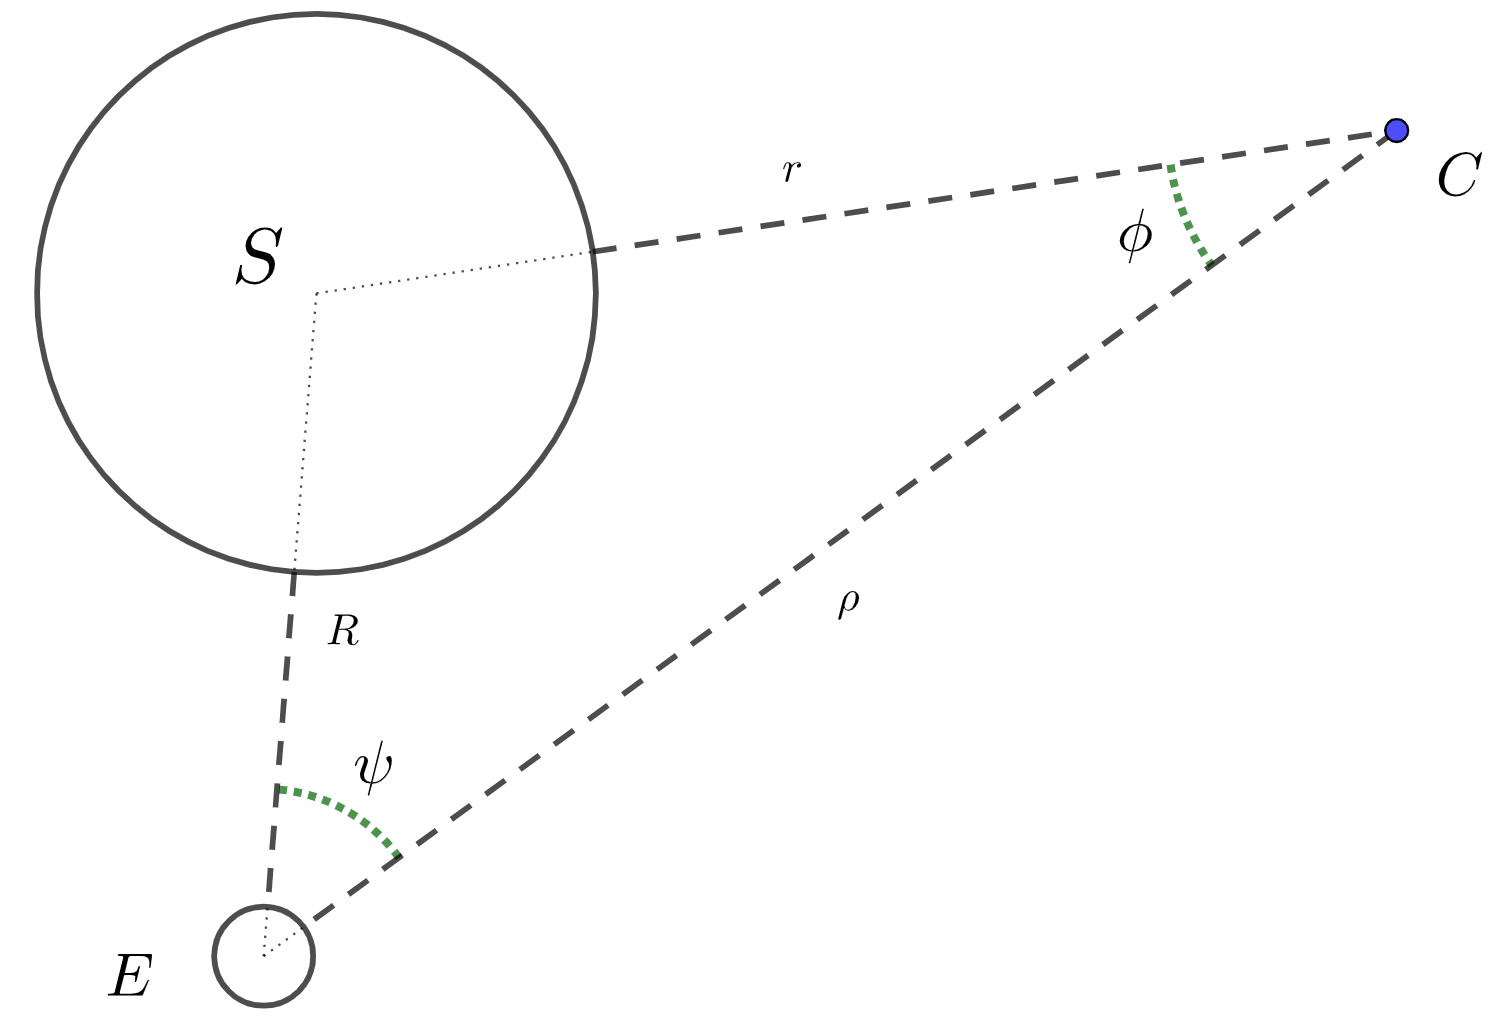
\includegraphics[scale=0.15]{images/notation_angles.png}
\caption{Triángulo formado por $S$, $E$ y $C$ junto a las distancias y ángulos generados.}
\label{fig:notation_angles}
\end{figure}

A partir de la figura superior, y junto al teorema de los senos ($\ddfrac{a}{\sin{\alpha}}=\ddfrac{b}{\sin{\beta}}=\ddfrac{c}{\sin{\gamma}}$), podemos deducir las siguientes ecuaciones:
\begin{align}
\left\{
\begin{array}{l}
	R\cos{\phi}=X\lambda+Y\mu+Z\nu\\
	\rho=R\ddfrac{\sin{(\psi+\phi)}}{\sin{\phi}}\; \; \; \; \; \cite{ASA}\\
	r=R\ddfrac{\sin{\psi}}{\sin{\phi}}
\end{array}
\right.
\label{eq:triangle_relations}
\end{align}

Sustituyendo dichas ecuaciones en la ecuación de $\rho$ en \eqref{eq:rho_values} obtenemos:
\[
R\sin{\psi}\cos{\phi}+\left(R\cos{\psi}-\ddfrac{D_1}{DR^3}\right)\sin{\phi}=\ddfrac{-D_1}{DR^3\sin^3{\psi}}\sin^4{\phi}
\]

Con el fin de simplificar esta expresión, definamos las siguientes expresiones:
\begin{align}
\left\{
\begin{array}{l}
	N\sin{m}=R\sin{\psi}\\
	N\cos{m}=R\cos{\psi}-\ddfrac{D_1}{DR^3}\\
	M=\ddfrac{-NDR^3\sin^3{\psi}}{D_1}
\end{array}
\right.
\label{eq:to_simplify}
\end{align}

El signo de $N$ será elegido de tal manera que $M$ sea positivo; fijado el signo, las dos primeras ecuaciones de \eqref{eq:to_simplify} determinarán unívocamente los valores $N$ y $m$, y la expresión que queríamos simplificar pasa a ser simplemente:
\begin{align}
\def\arraystretch{2}
\begin{array}{c}
	N\sin{m}\cos{\phi}+N\cos{m}\sin{\phi}=N\sin{(\phi+m)}=\ddfrac{N}{M}\sin^4{\phi} \Longrightarrow\\
	\Longrightarrow\sin^4{\phi}=M\sin{(\phi+m)}
\end{array}
\label{eq:phi_solution}
\end{align}

El valor para $M$ y $m$ serán conocidos cuando $M$ sea positivo. Busquemos ahora la solución de esta ecuación para $\phi$; dado que $\rho=0$ y $r=R$ es una solución al problema, podremos asegurar que $\phi=\pi-\psi$ es una solución válida, aunque no es de valor práctico dado que ésta corresponde a la posición del observador en la Tierra. Por tanto, dado que la solución ha de pertenecer al problema físico y que nos encontramos en un triángulo, podemos asegurar que:
\[
\phi<\pi-\psi
\]

Así, las soluciones de \eqref{eq:phi_solution} han de ser las intersecciones entre las curvas que definen las ecuaciones de la izquierda y de la derecha, es decir, la intersección entre:
\[
\left\{
\begin{array}{l}
y_1=\sin^4{\phi}\\
y_2=M\sin{(\phi+m)}
\end{array}
\right.
\]

Si el valor de $m$ es negativo cercano a cero y $M$ es ligeramente menor que 1, podemos ver la relación entre ambas curvas $y_1$, $y_2$ en la figura inferior:

\begin{figure}[H]
\centering
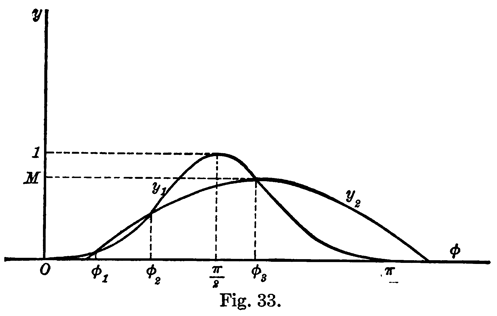
\includegraphics[scale=0.5]{images/fig_33.png}
\caption{Representación gráfica de $y_1$ e $y_2$ ($\frac{D_1}{D}>0$).}
\label{fig:y1_y2_graph_positive}
\end{figure}

En dicha imagen podemos ver que obtenemos tres intersecciones de las curvas, correspondientes cada una a una solución de \eqref{eq:phi_solution} y con $\phi_1<\phi_2<\phi_3$.\\

Discutamos ahora según el signo de $\frac{D_1}{D}$ los valores de $r$, $R$ y $m$. Comencemos considerando que $\frac{D_1}{D}$ es positivo. Es claro que $\rho$ y $r$ han de ser positivos, por lo que deducimos de la primera ecuación de \eqref{eq:rho_values} que $r$ ha de ser mayor que $R$. Por tanto, como $\psi$ ha de ser menor que 180º (pues estamos en un triángulo), utilizando las ecuaciones \eqref{eq:to_simplify} tenemos:
\[
\def\arraystretch{2}
\begin{array}{l}
M=\ddfrac{-NDR^3\sin^3{\psi}}{D_1}>0 \Longrightarrow N<0 \\
R\sin{\psi}>0 \Longrightarrow N\sin{m}>0 \Longrightarrow \sin{m}<0 \Longrightarrow m\in(\pi,2\pi)
\end{array}
\]

Por tanto, $N$ es negativo y $m$ estará en el tercer o cuarto cuadrante.\\

Si $m$ está en el cuarto cuadrante, la rama ascendente de la curva $y_2$ atraviesa el eje de abscisas $\phi$ en el primer cuadrante y, si $M<1$, las relaciones entre las dos curvas serán las que podemos ver en la figura \ref{fig:y1_y2_graph_positive}. Si el valor de $m$ es cercano a 180º tendremos tres soluciones disponibles $\phi_1$, $\phi_2$, $\phi_3$, una de las cuales corresponderá al observador ($\phi_i=\pi-\psi$). Discutamos según cuál de las tres soluciones toma este valor:
\begin{itemize}
\item Si $\phi_3=\pi-\psi$, las otras dos soluciones cumplirán todas las condiciones del problema, no pudiendo determinar cuál de las dos pertenece a la órbita real del cuerpo observado (siempre que no tengamos información adicional). Pero, podría darse el caso de que en estas condiciones los valores de $r$ y $\rho$ proporcionados por la solución $\phi_1$ fueran demasiado grandes como para que el objeto fuera visible para el observador, llegando así a la conclusión de que $\phi_2$, el cuál proporcionaría un $r$ más pequeño, pertenecería al problema físico.
\item Si $\phi_2=\pi-\psi$, se sigue del hecho de que $\phi<\pi-\psi$ que la solución ha de ser $\phi_1$.
\item Si $\phi_1=\pi-\psi$, entonces el problema no tendría solución dado que cualquiera de las otras dos soluciones sería mayor que $\pi-\psi$.
\end{itemize} 

A medida que la rama ascendente de la curva $y_2$ se mueve hacia la derecha, es decir, fijando $M$ y haciendo crecer $\phi_3$, las soluciones $\phi_1$ y $\phi_2$ tienden a coincidir, y en estas condiciones, que corresponderían a $m$ lejos de 180º en el tercer o cuarto cuadrante, el problema no tendría solución. Por tanto:
\begin{quote}
\textit{Si $\frac{D_1}{D}>0$, la distancia $r$ es mayor que $R$, el ángulo $m$ estará en el cuarto cuadrante y disponemos de dos o tres soluciones del problema físico en función de que $\phi_2$ o $\phi_3$ sea igual a $\pi-\psi$.}\\
\end{quote}

Veamos ahora el caso contrario. 

\begin{figure}[H]
\centering
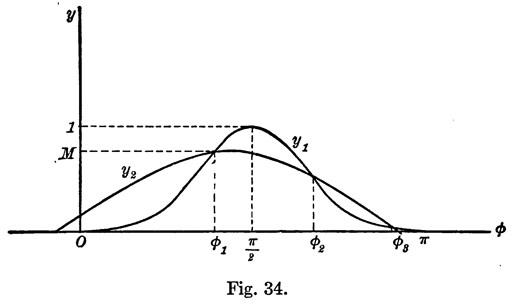
\includegraphics[scale=0.55]{images/fig_34.png}
\caption{Representación gráfica de $y_1$ e $y_2$ ($\frac{D_1}{D}<0$).}
\label{fig:y1_y2_graph_negative}
\end{figure}

Supongamos que $\frac{D_1}{D}$ es negativo, de tal manera que, procediendo como en el caso positivo, llegamos a que $r<R$ y que $m$ está en el primer o segundo cuadrante. Si $m$ está en el primer cuadrante, la rama descendente de la curva $y_2$ atraviesa el eje de abscisas $\phi$ en el segundo cuadrante, y para un $m$ pequeño y $M<1$, las relaciones entre las dos curvas serán las que podemos ver en la gráfica \ref{fig:y1_y2_graph_negative}. En este caso, la solución será única o doble en función de que $\phi_2$ o $\phi_3$ valgan $\pi-\psi$. Por último, si $m$ estuviera en el segundo cuadrante, la parte descendente de $y_2$ cortaría el eje de abscisas en el primer cuadrante, por lo que $\phi_2$ y $\phi_3$ no serían reales y el problema no tendría solución. Así, tenemos que:
\begin{quote}
\textit{Si $\frac{D_1}{D}<0$, la distancia $r$ es menor que $R$, el ángulo $m$ estará en el primer cuadrante y disponemos de dos o tres soluciones del problema físico en función de que $\phi_2$ o $\phi_3$ sea igual a $\pi-\psi$.}\\
\end{quote}



\subsection{\normalfont{\textit{Unicidad de la solución}}}
\label{subsec:unicidad}
Tal y como hemos visto en la sección anterior, la solución del problema físico será única si $\phi_2=\pi-\psi$, independientemente del signo de $\frac{D_1}{D}$; en otro caso, la solución será doble o no existirá. Sea $\varepsilon>0$ un valor pequeño y supongamos que $\phi=\pi-\psi+\varepsilon$. Entonces, si $\frac{D_1}{D}$ es positivo, podemos ver en la gráfica \ref{fig:y1_y2_graph_positive} que la diferencia $y_1-y_2$ es positiva cuando $\phi=\phi_2+\varepsilon$; y si $\frac{D_1}{D}$ es negativo, podemos ver en la gráfica \ref{fig:y1_y2_graph_negative} que $y_1-y_2$ es negativo cuando $\phi=\phi_2+\varepsilon$.\\

Sabemos que las funciones $y_1$ e $y_2$ son analíticas, y que la suma, el producto y la composición de funciones analíticas es analítica. Por tanto, $y_1-y_2$ es analítica y podremos expandirla como serie de potencias en $\varepsilon$ cuando $\phi=\pi-\psi+\varepsilon$. Así, tenemos la siguiente expresión:
\begin{align}
\begin{array}{l}
y_1-y_2=[\sin^4{(\pi-\psi)}-M\sin{(\pi-\psi+m)}]+\\+[4\sin^3{(\pi-\psi)}\cos{(\pi-\psi)}-M\cos{(\pi-\psi+m)}]\epsilon+...
\end{array}
\label{eq:y1_y2_serie}
\end{align}

\noindent donde hemos tomando $\varepsilon_0=0$ dado que $\phi=\pi-\psi$ es una solución del problema. Pasemos a simplificar esta expresión y reducir el coeficiente de $\varepsilon$ utilizando las ecuaciones \eqref{eq:to_simplify} y \eqref{eq:phi_solution}:
\[
\def\arraystretch{2}
\begin{array}{ll}
& [\sin^4{(\pi-\psi)}-\sin^4{(\pi-\psi)}]+[-4\sin^3{(\pi-\psi)}\cos{\psi}+M\cos{(-\psi+m)}]=\\
= & 0 + \left[\ddfrac{4MD_1}{NDR^3}\cos{\psi}+M(\cos{\psi}\cos{m}+\sin{\psi}\sin{m})\right]=\\
= & \ddfrac{4MD_1}{NDR^3}\cos{\psi}+M\left(\ddfrac{R\cos^2{\psi}}{N}-\ddfrac{D_1\cos{\psi}}{NDR^3}+\ddfrac{R\sin^2{\psi}}{N}\right)=\\
= & \ddfrac{4MD_1}{NDR^3}\cos{\psi}-\ddfrac{MD_1}{NDR^3}\cos{\psi}+\ddfrac{MR}{N}(\cos^2{\psi}+\sin^2{\psi})=\\
= & \ddfrac{MR}{N}\left(1+\ddfrac{3D_1}{DR^4}\cos{\psi}\right)
\end{array}
\]

\vspace{0.4cm}

Por tanto, la serie pasa a ser:
\begin{align}
y_1-y_2=\ddfrac{MR}{N}\left(1+\ddfrac{3D_1}{DR^4}\cos{\psi}\right)\varepsilon+...
\label{eq:y1_y2_serie2}
\end{align}

Así, conociendo que $MR>0$, llegamos a la conclusión de que la condición para que el problema físico tenga solución única es:
\begin{align}
\left\{
\def\arraystretch{2}
\begin{array}{l}
	\ddfrac{1}{N}\left[1+\ddfrac{3D_1}{DR^4}\cos{\psi}\right]>0 \; \; \; \; \text{si} \; \; \; \; \ddfrac{D_1}{D}>0\\
	\ddfrac{1}{N}\left[1+\ddfrac{3D_1}{DR^4}\cos{\psi}\right]<0 \; \; \; \; \text{si} \; \; \; \; \ddfrac{D_1}{D}<0
\end{array}
\right.
\label{eq:condicion_unicidad}
\end{align}

Dado que todos los valores de estas ecuaciones están dados por simples observaciones, no será necesario resolver la ecuación \eqref{eq:phi_solution} para determinar la unicidad de la solución.












\newpage

\begin{thebibliography}{99}
\bibitem{moulton} \textsc{Forest Ray Moulton}, \textsc{An Introduction to Celestial Mechanics}, \textit{second edition}.

\bibitem{ortega} \textsc{R. Ortega, A.J. Ureña}, \textsc{Introducción a la Mecánica Celeste}.

\bibitem{right_ascension_declination} \textsc{Sky \& Telescope}, \textsc{Right Ascension and Declination: Celestial Coordinates For Beginners}, \url{https://skyandtelescope.org/astronomy-resources/right-ascension-declination-celestial-coordinates/}

\bibitem{ASA} \textsc{Solution of triangles}, \url{https://en.wikipedia.org/wiki/Solution_of_triangles#A_side_and_two_adjacent_angles_given_(ASA)}

\end{thebibliography}

\end{document}


